\documentclass[
	%a4paper, % Use A4 paper size
	letterpaper, % Use US letter paper size
]{jdf}

\addbibresource{references.bib}

\author{Kha Kein “Luke” Cheng}
\email{Kcheng314@gatech.edu}
\title{Final Project}
\usepackage{caption}
\usepackage{tabularx}
\usepackage{float}
\usepackage{xurl} 
\usepackage{hyperref}
\captionsetup{justification=centering}
\begin{document}
%\lsstyle

\maketitle

\section{Task 1: Find a Recent Public Artifact Addressing AI Misuse }
\subsection{Public Artifact}
\begin{itemize}
    \item Title: "AI Hiring Tools Can Yield Racial Bias and Systemic Rejection”
    \item Released: May 26, 2026 
    \item Link: https://hai.stanford.edu/news/ai-hiring-tools-can-yield-racial-bias-and-systemic-rejection
\end{itemize}

\subsection{Application/Scenario/Domain of Misuse}
Automated Candidate Resume Screening

\subsection{Regulated Domain/Protected Class}
\begin{itemize}
    \item Regulated Domain: Employment
    \item Protected Classes Impacted: Race and Ethnicity
\end{itemize}

\subsection{Evidence}
https://news.stanford.edu/stories/2026/06/ai-hiring-tools-racial-bias-research


\section{Task 2: Summary of Bias in Public Artifact}
This report shows how automated hiring tools used by major companies are biased against job seekers with certain ethinicity. When filtering through applicants, these tools tend to \textbf{filter out Black and Asian candidates while favoring White candidates}. Instead of filtering based on their qualifications, the algorithm relies on older, biased data and clues like test games or educational background. As a result, qualified minority applicants are frequently rejected before a human recruiter ever sees their application.

Furthermore, the report shows how \textbf{broad summary statistics} can easily hide this discrimination and mislead readers. Looking at hiring numbers across an entire company might make the system seem fair, but breaking down it down job by job reveals clear violations of employment fairness laws. To make it worse, over 150 top companies use the same hiring software, thus a single flaw in the system gets repeated everywhere. For example,If a candidate is mistakenly rejected by this algorithm once, they  will end up getting rejected as well from jobs across other companies as they are using the same tools.



\begin{figure}[H]
	\centering
	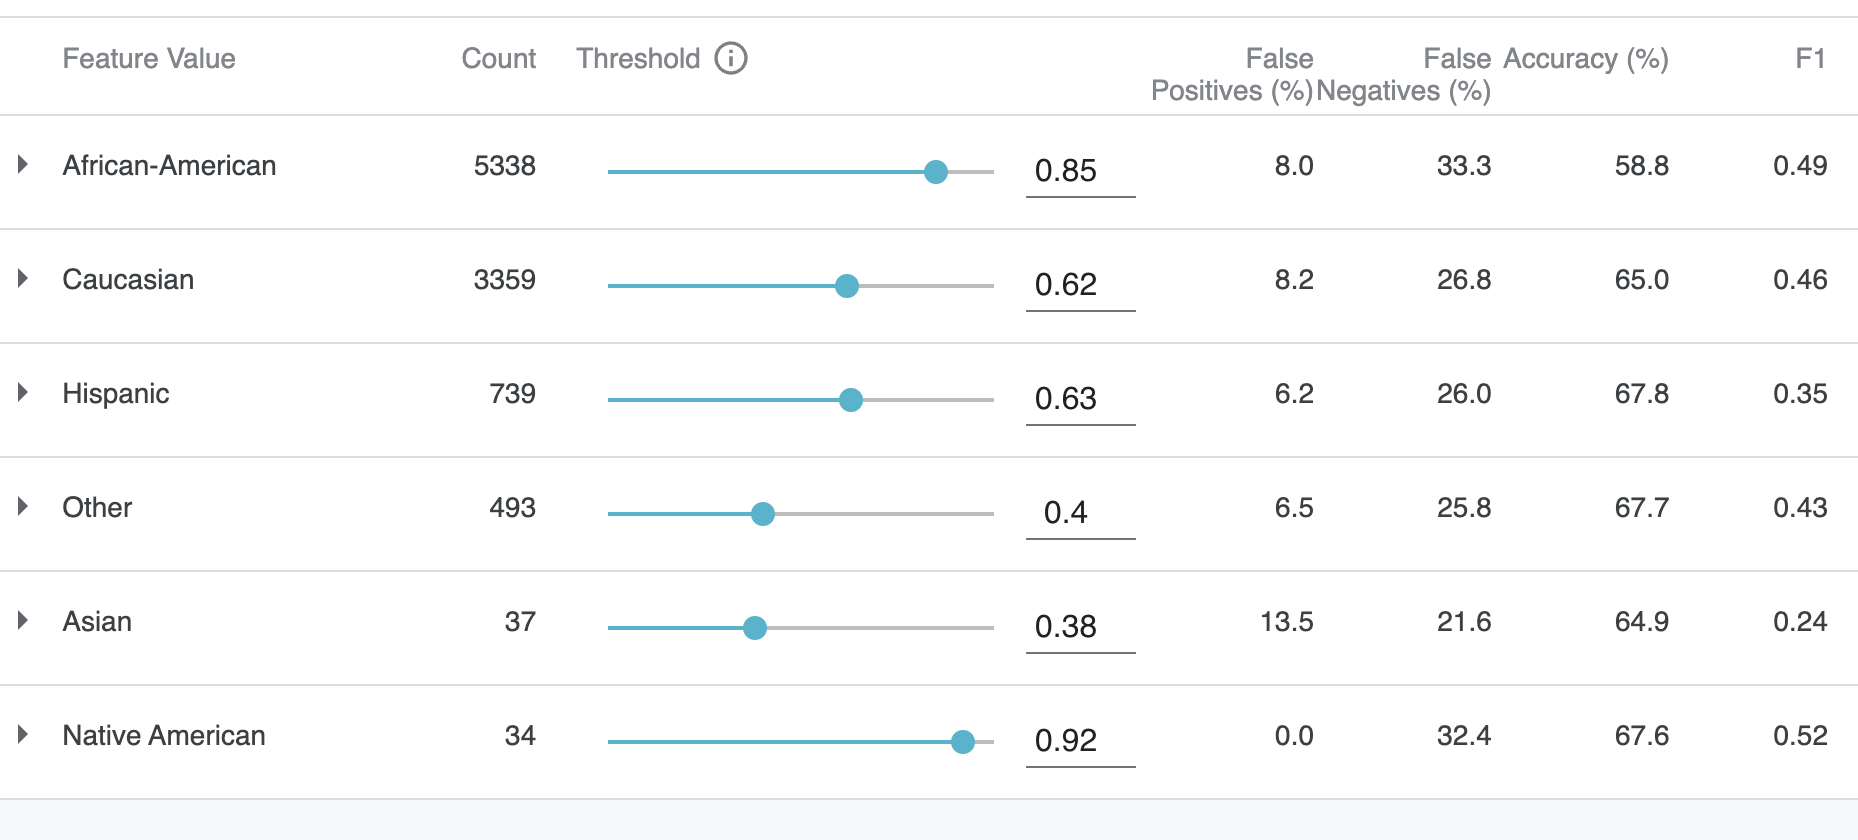
\includegraphics[height=6cm]{Figures/figure2.png}
	\caption{Sex vs G2\_Pass}
	\label{fig:figure_2}
\end{figure}

\begin{thebibliography}{2}

\bibitem{blow2023comprehensive}
Blow, C. H., Qian, L., Gibson, C., Obiomon, P., \& Dong, X. (2023). ``Comprehensive validation on reweighting samples for bias mitigation via AIF360.'' \textit{arXiv preprint arXiv:2312.12560}. 
\textsc{url}: \url{https://arxiv.org/abs/2312.12560}.

\end{thebibliography}
\printbibliography[heading=none]

\end{document}